%% V. Results, organised by research question. Input by access.tex.
\section{Results}
\label{sec:results}

\subsection{Gates, Retention and Feature Structure}
On ds001787 the locked artefact rule retained 22 of 40 sessions (12 experienced, 10 novices, from 16 subjects) with 554 rated probes and a median of 30\,\% missing epochs. The loss of 45\,\% is below the stop threshold of 50\,\% but is not random: it is driven by muscle artefact on temporal channels and by three subjects with globally high amplitude. On OSF 3uszv the adaptive rule retained 48 of 58 sessions (25 experienced, 23 novices) with 1,838 rated probes; the ten excluded sessions had more than 40\,\% missing epochs. The probe windows alone cover 34\,\% of an OSF session (a response takes 17~s on average, every 77~s, and every epoch that overlaps a probe window is masked), so the retained sessions still have a median of 36\,\% missing epochs. The DMN feature had temporal structure on both datasets (median lag-1 autocorrelation of $y_A$ 0.42 and 0.77; stop criterion K2 not triggered); the complexity feature had almost none on ds001787 (0.10) and some on OSF 3uszv (0.20). All eight gates passed in order. Fig.~\ref{fig:sessions} shows one retained session of each dataset as the fitted model sees it.

\begin{figure*}[t]
\centering
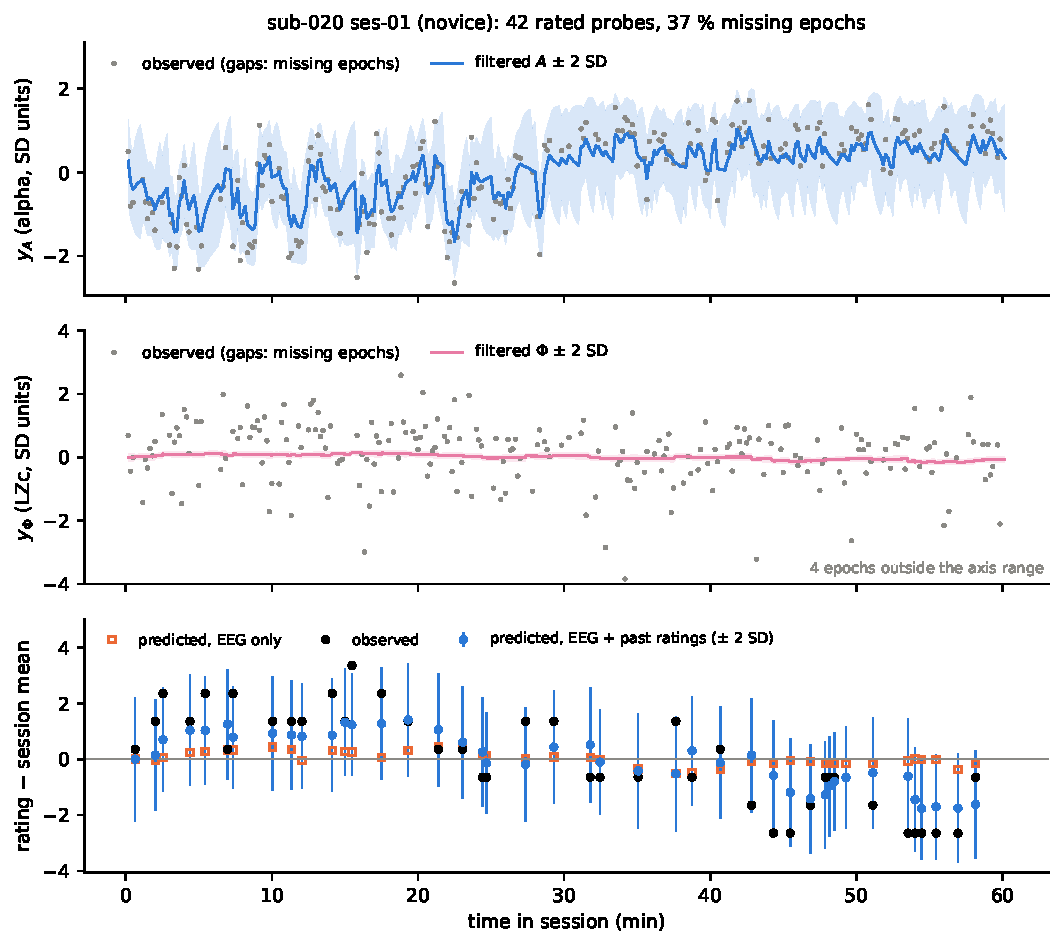
\includegraphics[width=0.49\textwidth]{fig9_realdata_session.pdf}\hfill
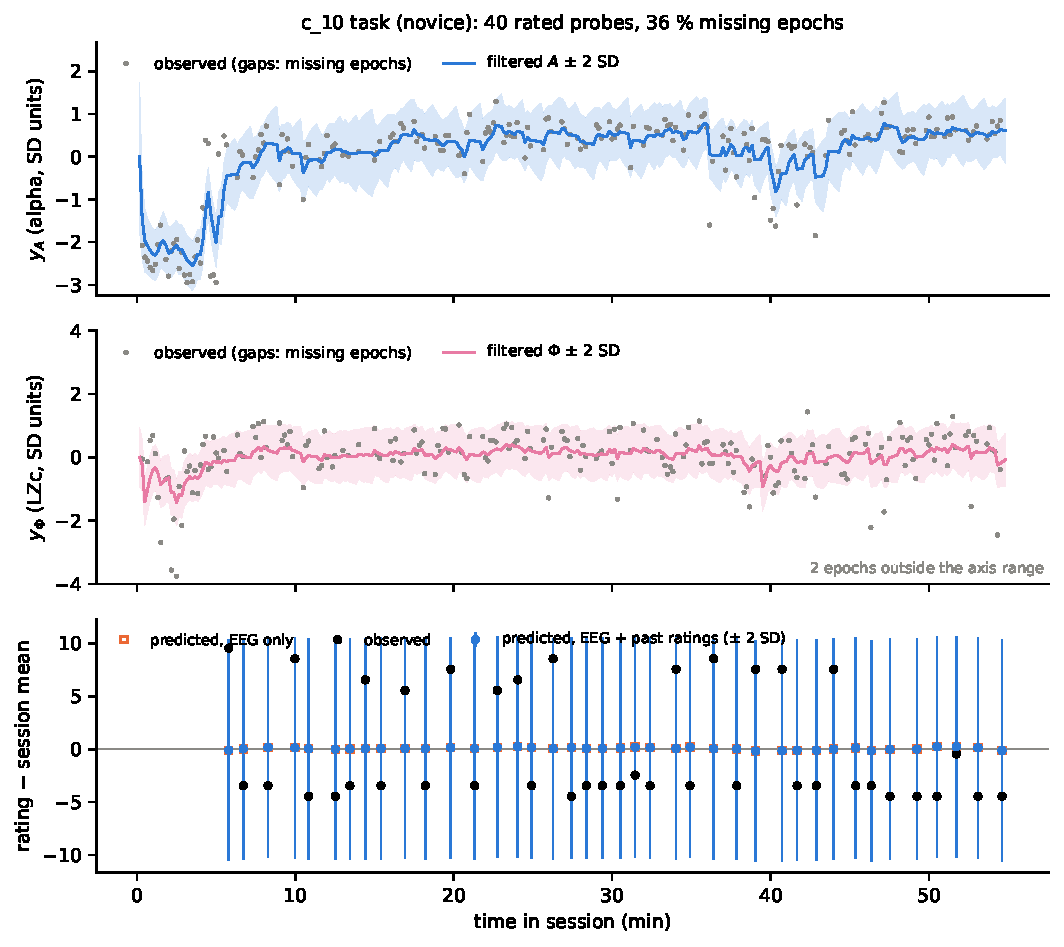
\includegraphics[width=0.49\textwidth]{fig11_osf_session.pdf}
\caption{\textbf{One retained session of each dataset filtered with M1 at the pooled estimate (in sample).} Left: ds001787, sub-020 ses-01 (novice); right: OSF 3uszv, c\_10 (novice); in each case the retained session with the most rated probes. Top: DMN proxy $y_A$ and the filtered $A\pm2$ SD. Middle: integration proxy $y_\Phi$ and the filtered $\Phi\pm2$ SD; on ds001787 the filtered $\Phi$ hardly moves because $y_\Phi$ is almost pure noise, on OSF 3uszv it fluctuates on a scale of tens of seconds; a few outlying epochs lie outside the axis. Bottom: ratings centred within session, with one-step-ahead predictions from EEG and past ratings ($\pm2$ SD) and from EEG alone. Gaps are missing epochs. On OSF 3uszv the alpha proxy drifts over minutes, with level shifts near 5 and 40~min, and the ratings alternate between about $+7$ and $-5$ without serial dependence, so that every prediction stays at the session mean.}
\label{fig:sessions}
\end{figure*}

\subsection{Predicted and Achieved Errors (RQ1)}
Fig.~\ref{fig:errors} is the main result. For the seven scale-free parameters of M1 it shows, on each dataset, the CRB computed before the lock, the Fisher standard error at the estimate, the bootstrap RMSE and the observed-information standard error. Table~\ref{tab:errors} gives the numbers for the two rate constants. On ds001787 the bound for $\kinh$ computed before any EEG was seen (9.1\,\%) and the bound recomputed on the retained sessions at the measured signal-to-noise ratio (13.3\,\%) bracket the 9.9\,\% achieved, and the bootstrap reproduces the Fisher value (ratio 0.98). On OSF 3uszv the denser probing and longer sessions give a smaller bound, 6.7\,\%, and the achieved Fisher error is 8.5\,\% with a bootstrap ratio of 1.03; the bootstrap-to-Fisher ratios are 0.98--1.69 on ds001787 and 1.00--1.08 on OSF 3uszv over all ten parameters, so gates E2 and F2 pass. Hypothesis H1 is supported under its preregistered Fisher criterion on both datasets. In Fisher terms the design analysis was accurate on ds001787 and somewhat optimistic on OSF 3uszv, where the achieved error exceeds the bound recomputed on the retained sessions by 15\,\%; both are well inside the factor of two with which the bound was validated in simulation.

\begin{figure*}[t]
\centering
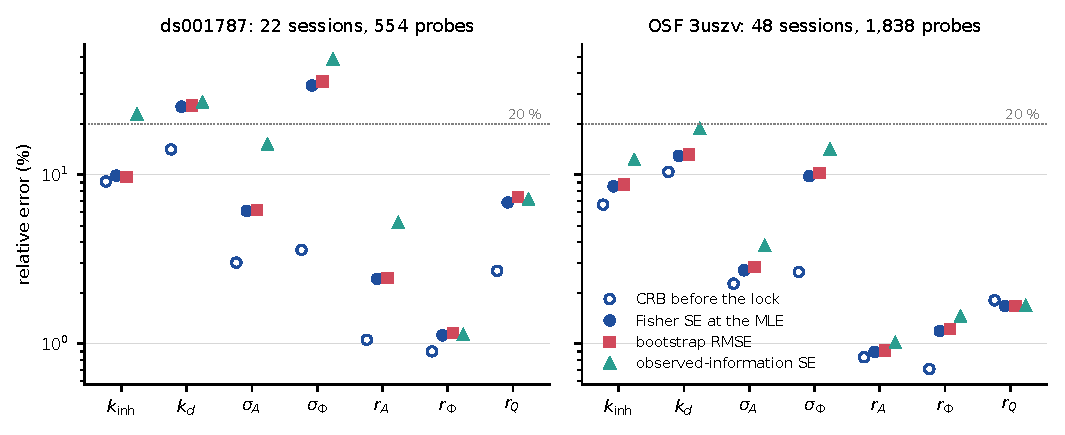
\includegraphics[width=0.95\textwidth]{fig1_pred_vs_achieved.pdf}
\caption{\textbf{Predicted and achieved relative errors of the scale-free parameters of M1 on the two datasets.} Open circles: Cram\'er--Rao bound from the exact Fisher information at the nominal parameters on the real probe schedules, computed before each lock. Filled circles: Fisher standard error at the maximum-likelihood estimate. Squares: root-mean-square error of 200 parametric-bootstrap refits. Triangles: standard error from the observed information (numerical Hessian). The dotted line is the 20\,\% criterion of hypothesis H1. For $\kinh$ the first three numbers agree on both datasets (largest over smallest 1.08 and 1.32); for $\kd$ the Fisher error exceeds the bound computed before the lock by a factor of 1.8 on ds001787 and 1.2 on OSF 3uszv; the observed-information error of the alpha-power channel ($\kinh$, $\sA$, $\rA$) exceeds the Fisher error by a factor of 2.1--2.5 on ds001787 and 1.1--1.4 on OSF 3uszv.}
\label{fig:errors}
\end{figure*}

\begin{table}[t]
\caption{\textbf{Three error numbers for the two rate constants (per minute), as relative errors in percent.} CRB: before the lock on all real designs, on the retained designs, and on these with $\rA$ at the measured signal-to-noise ratio. SE at the MLE: expected Fisher information, observed information, and profile likelihood. RMSE: 200 bootstrap refits; ratio: RMSE over Fisher SE (gate E2/F2).}
\label{tab:errors}
\centering\scriptsize
\setlength{\tabcolsep}{2.2pt}
\begin{tabular}{llrrrrrrrrr}
\toprule
 & & & \multicolumn{3}{c}{CRB} & \multicolumn{3}{c}{SE at the MLE} & & \\
\cmidrule(lr){4-6}\cmidrule(lr){7-9}
Dataset & Par. & Est. & lock & kept & SNR & Fisher & obs. & prof. & RMSE & ratio \\
\midrule
ds001787  & $\kinh$ & 1.32  & 9.1  & 12.3 & 13.3 & 9.9  & 22.8 & 21.9 & 9.7  & 0.98 \\
          & $\kd$   & 0.200 & 14.1 & 19.0 & 19.1 & 25.3 & 26.7 & 26.6 & 25.7 & 1.01 \\
OSF 3uszv & $\kinh$ & 0.140 & 6.7  & 7.4  & 7.4  & 8.5  & 12.2 & 11.8 & 8.8  & 1.03 \\
          & $\kd$   & 1.58  & 10.4 & 11.5 & 11.5 & 12.9 & 18.7 & 18.3 & 13.2 & 1.02 \\
\bottomrule
\end{tabular}
\end{table}

\subsection{The Misspecification Signature (RQ1)}
The observed information tells a different story for the DMN channel. On ds001787 the numerical Hessian gives 22.8\,\% for $\kinh$ and the profile likelihood 21.9\,\%, more than twice the Fisher value; the same factor, 2.1--2.5, appears for $\sA$ and $\rA$, whereas for $\kd$, $\rPhi$ and $\rQ$ observed and expected information agree within 6\,\%. On a dataset simulated from $\hat\thetav$ on the same 22 designs the factor for $\kinh$, $\sA$ and $\rA$ is 1.05--1.07. A gap confined to one channel and absent under the fitted model is the signature of misspecification of that channel: posterior alpha power is not fully described by one Ornstein--Uhlenbeck process plus white noise. On OSF 3uszv the signature is present but weaker, 1.43 for $\kinh$, 1.39 for $\sA$ and 1.13 for $\rA$ against 0.93--0.99 on simulated data, and it is no longer confined to the alpha channel (1.45 for $\kd$, 1.44 for $\sPhi$); the replication check R2, which required the factor to exceed 1.5, is not met. Fig.~\ref{fig:profiles} shows the profiles: on ds001787 the profile of $\kinh$ is about twice as wide as the Fisher quadratic while that of $\kd$ follows it; on OSF 3uszv the profiles of $\kinh$ and $\kd$ are 1.4 times wider than the quadratic, and the profile of $\kappa$ is asymmetric. Under the likelihood-based criterion H1 is therefore not supported on ds001787 (21.9\,\%, just above 20\,\%) and supported on OSF 3uszv (11.8\,\%). We report the profile interval as the uncertainty of $\kinh$ throughout.

\begin{figure*}[t]
\centering
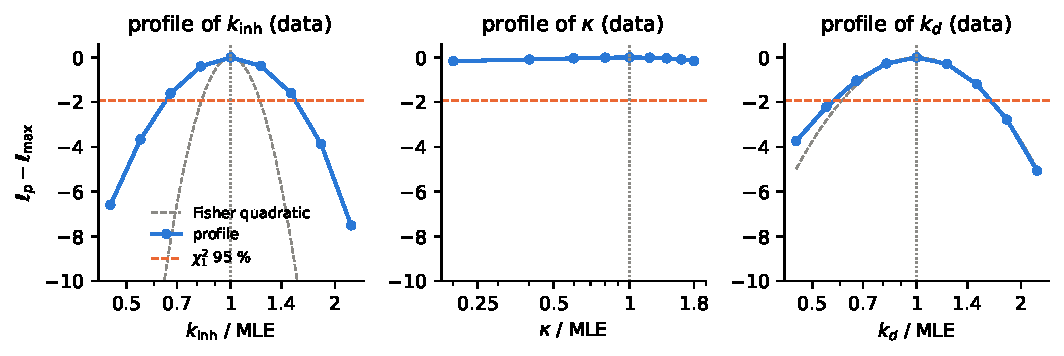
\includegraphics[width=0.82\textwidth]{fig10_realdata_profiles.pdf}\\[3pt]
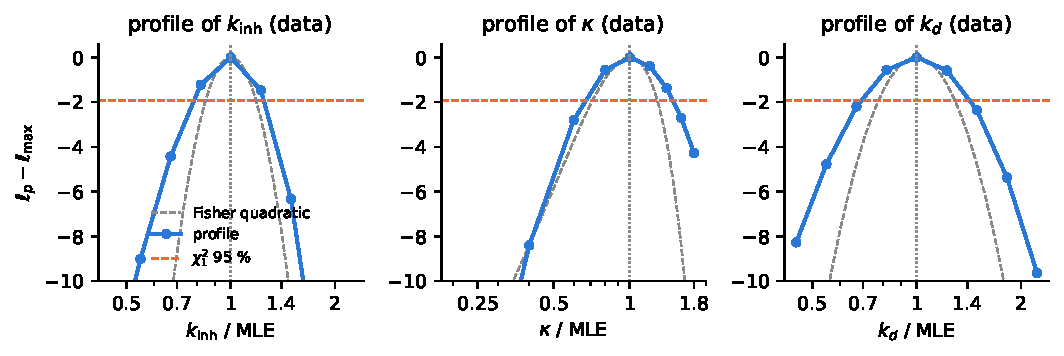
\includegraphics[width=0.82\textwidth]{fig12_osf_profiles.pdf}
\caption{\textbf{Profile log-likelihoods of the three rate constants, all other parameters re-optimised at each point.} Top: ds001787; bottom: OSF 3uszv. Grey dashed: quadratic approximation implied by the expected Fisher information at the maximum-likelihood estimate; orange: $\chi^2_1$ 95\,\% threshold. On ds001787 the profile of $\kinh$ is about twice as wide as the quadratic (95\,\% interval 0.86--2.02~min$^{-1}$), that of $\kd$ follows it, and that of $\kappa$ is flat because $\hat\kappa\approx0$. On OSF 3uszv the profile of $\kinh$ is 1.38 times wider than the quadratic (0.110--0.175~min$^{-1}$), that of $\kd$ 1.4 times, and the profile of $\kappa$, which is negative, is asymmetric ($-0.50$ to $-0.23$).}
\label{fig:profiles}
\end{figure*}

\subsection{Estimates}
Table~\ref{tab:compare} places the two fits side by side. On ds001787 the DMN proxy relaxes fast, $1/\hat k_{\mathrm{inh}}=0.76$~min (profile interval 0.49--1.17~min), against the nominal 5~min of the design analysis, and the latent integration variable slowly, $1/\hat k_d=5.0$~min (3.1--8.7~min); the coupling $\kappa$ is not distinguishable from zero. On OSF 3uszv the DMN proxy is slow, $1/\hat k_{\mathrm{inh}}=7.1$~min (5.7--9.1~min), nine times the ds001787 value, and the integration variable is fast, $1/\hat k_d=0.63$~min (0.45--0.91~min), eight times faster than before: the two time constants have exchanged places, and R1 fails by a factor of nine. The coupling is now determined and negative, $\hat\kappa=-0.33$ ($-0.50$ to $-0.23$). The proxies differ in quality between the datasets. On ds001787 the DMN channel has a signal-to-noise ratio of 1.11 against a nominal 1.58 and the integration channel 0.06 against a nominal 2.4: the spectrum-controlled complexity measure carries almost no slow signal. On OSF 3uszv the DMN channel has the nominal ratio (1.57) and the integration channel 0.54, eight times its ds001787 value.

\begin{table*}[t]
\caption{\textbf{The two preregistered fits side by side.} Time constants in minutes with 95\,\% profile intervals; gains with Fisher 95\,\% intervals and per unit of the within-session SD of the ratings (1.11 and 5.22). SE of $\kinh$: CRB before the lock, Fisher, observed information, profile likelihood. Obs/exp: observed over expected SE on the data (in parentheses: on data simulated from the fit). \mbox{\mathversion{normal}$\Delta$}LPD: out-of-sample log predictive density of M1 minus N2 (EEG only) and minus N1 (EEG and past ratings). Group difference: $\log\kinh$, experienced minus novice fit, Wald 95\,\% interval. Meta-analysis: random-effects $1/\kinh$ over the subjects with a finite SE and the between-subject SD $\tau$ of $\log\kinh$. Sensitivity: locked variants that keep the sign of $\alpha$, the sign of $\beta$ and the profile interval of $1/\kinh$.}
\label{tab:compare}
\centering\footnotesize
\setlength{\tabcolsep}{4pt}
\begin{tabular}{lll}
\toprule
 & ds001787 & OSF 3uszv \\
\midrule
Sessions retained / recorded; subjects   & 22 / 40; 16 & 48 / 58; 48 \\
Rated probes; probe interval; session    & 554; 1.6 min; 45 min & 1,838; 77 s; 57 min \\
Rating scale; within-session SD          & $-3$ to $3$; 1.11 & $-7$ to $7$; 5.22 \\
$1/\kinh$ (min)                          & 0.76 [0.49, 1.17] & 7.1 [5.7, 9.1] \\
$1/\kd$ (min)                            & 5.0 [3.1, 8.7] & 0.63 [0.45, 0.91] \\
$\kappa$                                 & $\approx0$, flat profile & $-0.33$ [$-0.50$, $-0.23$] \\
SNR of $y_A$; of $y_\Phi$                & 1.11; 0.06 & 1.57; 0.54 \\
SE of $\kinh$: CRB / Fisher / obs. / profile & 9.1 / 9.9 / 22.8 / 21.9\,\% & 6.7 / 8.5 / 12.2 / 11.8\,\% \\
Bootstrap RMSE / Fisher SE of $\kinh$    & 0.98 & 1.03 \\
Obs/exp SE: $\kinh$, $\sA$, $\rA$        & 2.30, 2.48, 2.14 (1.05--1.07) & 1.43, 1.39, 1.13 (0.93--0.99) \\
$\alpha$ [95\,\%]; per rating SD         & 13.1 [4.9, 21.3]; 11.8 & 0.79 [$-0.24$, 1.82]; 0.15 \\
$\beta$ [95\,\%]; per rating SD          & $-0.03$ [$-0.19$, 0.13]; $-0.02$ & 0.02 [$-0.34$, 0.38]; 0.00 \\
$\Delta$LPD vs N2; vs N1                 & $-0.010$; $-0.031$ & $+0.000$; $-0.001$ \\
Lag-1 autocorrelation of the ratings     & 0.22 & $-0.01$ \\
Group difference in $\log\kinh$          & $-1.19$ [$-1.56$, $-0.81$] & $+0.14$ [$-0.20$, 0.47] \\
Meta-analysis: $1/\kinh$; $\tau$; subjects & 0.95 [0.40, 2.26]; 1.19; 9 & 3.3 [2.0, 5.7]; 1.49; 35 \\
Ljung--Box median $p$: $y_A$, $y_\Phi$   & 0.27, 0.40 & 0.06, 0.42 \\
Sensitivity: $\alpha$, $\beta$, $1/\kinh$ kept & 6/6, 4/6, 4/6 & 5/6, 1/6, 4/6 \\
Gates                                    & E0--E3 passed & F0--F3 passed \\
\bottomrule
\end{tabular}
\end{table*}

\subsection{Gains and Out-of-Sample Prediction (RQ2)}
On ds001787 the gain from the integration variable to the rating is positive, $\hat\alpha=13.1$ (Fisher 95\,\% interval 4.9--21.3; no bootstrap replicate at or below zero), as hypothesis H3 predicted. Its meaning is limited: since $y_\Phi$ is essentially noise, the latent $\Phi$ is identified almost entirely by the ratings themselves, $\alpha$ and $\sPhi$ trade off (bootstrap correlation of $\log\sPhi$ and $\alpha$: $-0.83$), and only the contribution of $\Phi$ to the rating variance is well determined. On OSF 3uszv, where $\Phi$ is pinned by the complexity channel, $\hat\alpha=0.79$ with an interval that contains zero ($-0.24$ to $1.82$; 11 of 200 bootstrap replicates at or below zero): H3 is not supported. In units of the within-session rating SD the gain is 11.8 on ds001787 and 0.15 on OSF 3uszv. The DMN gain is $\hat\beta=-0.03$ ($-0.19$ to $0.13$) and $0.02$ ($-0.34$ to $0.38$): the sign asked for by H4 is not determined on either dataset, and posterior alpha power makes no detectable contribution to the ratings.

Table~\ref{tab:loso} gives the leave-one-session-out comparison of hypothesis H2. On ds001787, with EEG only, M1 predicts the ratings no better than the instantaneous regression N2; with EEG and past ratings it beats the running mean N3 but not the rating-only model N1, which has the best log predictive density and the smallest error of all models. The advantage over N3 therefore comes from the serial dependence of the reports (lag-1 autocorrelation 0.22), not from the EEG. On OSF 3uszv M1 is indistinguishable from N2 and N1 ($\Delta\mathrm{LPD}$ of $+0.0004$ and $-0.0006$), with a mean absolute error of 4.5--4.6 on a 14-point scale for every model but the running mean (4.7), and for a more basic reason: the ratings of this dataset have no serial dependence to predict (lag-1 autocorrelation $-0.01$), so past ratings do not help either, and their bimodal distribution is out of reach of a Gaussian read-out (Appendix~\ref{app:ppc}). H2 is not supported on either dataset.

\begin{table*}[t]
\caption{\textbf{Leave-one-session-out prediction of the ratings (hypothesis H2), (a) from EEG only and (b) from EEG and past ratings.} LPD: mean Gaussian log predictive density per probe; MAE: mean absolute error. \mbox{\mathversion{normal}$\Delta$}LPD: M1 minus null model with a session-level bootstrap 95\,\% interval. N2: instantaneous regression on $(y_A,y_\Phi)$; N1: M1 with the rating channel only; N3: running mean of past ratings.}
\label{tab:loso}
\centering\footnotesize
\setlength{\tabcolsep}{5pt}
\begin{tabular}{llrrrrr}
\toprule
 & Comparison & LPD M1 & LPD null & $\Delta$LPD [95\,\%] & MAE M1 & MAE null \\
\midrule
ds001787 & (a) vs N2 & $-1.546$ & $-1.541$ & $-0.010$ [$-0.039$, $0.017$] & 0.93 & 0.92 \\
(554 probes) & (b) vs N1 & $-1.472$ & $-1.421$ & $-0.031$ [$-0.103$, $0.009$] & 0.88 & 0.84 \\
 & (b) vs N3 & $-1.472$ & $-1.626$ & $+0.154$ [$0.083$, $0.233$] & 0.88 & 1.00 \\
\midrule
OSF 3uszv & (a) vs N2 & $-3.0746$ & $-3.0749$ & $+0.0004$ [$-0.0006$, $0.0014$] & 4.54 & 4.56 \\
(1,838 probes) & (b) vs N1 & $-3.0746$ & $-3.0740$ & $-0.0006$ [$-0.0018$, $0.0006$] & 4.54 & 4.55 \\
 & (b) vs N3 & $-3.0746$ & $-3.1445$ & $+0.0712$ [$0.0609$, $0.0815$] & 4.54 & 4.66 \\
\bottomrule
\end{tabular}
\end{table*}

\subsection{Groups and Subjects}
On ds001787, fitted separately, the experienced group has a smaller $\kinh$ than the novices (log difference $-1.19$, Wald 95\,\% interval $-1.56$ to $-0.81$), opposite to hypothesis H5. The two separate fits differ mainly in how the alpha-power variance is split between state and observation noise (signal-to-noise ratio 1.05 against 2.23), and $\kinh$ trades off against that split: when all other parameters are shared the log difference shrinks to $-0.18$ and the preregistered one-degree-of-freedom test is not significant ($\chi^2_1=3.3$, $p=0.068$), although the groups differ in some parameter ($\chi^2_{10}=41$). The groups also differ in sex and age (10 of 12 against 2 of 12 men, mean age 39 against 48 years). On OSF 3uszv, with 25 and 23 sessions, the group fits give $\hat k_{\mathrm{inh}}=0.154$ and $0.134~\mathrm{min^{-1}}$, a log difference of $+0.14$ ($-0.20$ to $0.47$; $\chi^2_1=2.67$, $p=0.10$), below the minimal detectable difference of 0.37: neither F-H5a nor F-H5b is supported, and the difference found on ds001787 does not recur. The groups differ in other parameters ($\chi^2_{10}=256$): in the novices the integration variable is fast and noisy ($1/\kd=0.33$~min, $\sPhi=1.1$) and loads positively on the reports ($\alpha=2.0$, $\beta=+0.75$); in the experienced practitioners it is slower ($1/\kd=0.89$~min, $\sPhi=0.68$) and both gains are near zero or negative ($\alpha=-0.15$, $\beta=-0.66$). Per-subject fits gave finite standard errors for 9 of 16 subjects on ds001787 and 35 of 48 on OSF 3uszv (for most of the others $\sPhi$ was estimated at zero). Their meta-analyses give DMN time constants of 0.95~min (0.40--2.26) and 3.3~min (2.0--5.7) with between-subject standard deviations of $\log\kinh$ of 1.19 and 1.49 log units ($I^2=0.92$ on both): the pooled fits describe an average practitioner at best.

\subsection{Model Checks and Sensitivity}
The innovations are close to white on ds001787 (median Ljung--Box $p=0.27$ for $y_A$ and $0.40$ for $y_\Phi$; four of 22 sessions below 0.01 for $y_A$) and less so on OSF 3uszv ($p=0.058$ for $y_A$, with 17 of 48 sessions below 0.01; $0.42$ for $y_\Phi$); the innovations of the two channels are uncorrelated on both (median 0.05), so the diagonal observation noise was kept. The posterior predictive check (Appendix~\ref{app:ppc}) reproduces the serial dependence of the ds001787 ratings (lag-1 autocorrelation 0.22, simulated 0.26, band 0.15--0.37) and the absence of serial dependence on OSF 3uszv ($-0.01$; simulated $-0.03$, band $-0.08$ to $0.02$), but not the skewed centre of the ds001787 distribution nor the bimodal OSF distribution, and on both datasets the experienced practitioners rate with a smaller spread than the pooled model implies (OSF: observed difference in within-session SD $-1.01$, simulated $-0.31$, band $-0.55$ to $-0.05$).

Table~\ref{tab:sens} lists the sensitivity analyses. On ds001787 $\alpha$ stays positive in all six locked variants, the sign of $\beta$ is kept in four, and $1/\kinh$ stays inside the profile interval in four: the frontal-theta proxy gives 4.0~min, and the variant with at most 20\,\% missing epochs keeps two sessions and is degenerate. On OSF 3uszv that variant retains no session, because the probe windows alone exceed 20\,\% in every session, an oversight of the preregistration, so six variants run; the sign of $\alpha$ is kept in five (it is negative with the aperiodic-exponent proxy), the sign of $\beta$ in one, and $1/\kinh$ stays inside the interval in four (frontal theta gives 17~min and per-session z-scoring 4.8~min). The 80\,\% rule is therefore met for the sign of $\alpha$ on both datasets and for nothing else, and the estimates are reported descriptively. One post-registration variant on OSF 3uszv, added after Fig.~\ref{fig:sessions} had been examined, masks the EEG before the first probe (the sessions begin with instructions and a practice probe, and the first bell comes after 6.8~min on average): the DMN time constant rises from 7.1 to 16~min, so the level shift of alpha at the start of the session is the fastest part of this proxy.

\begin{table*}[t]
\caption{\textbf{Sensitivity analyses: pooled estimates with time constants in minutes.} The fixed 150~$\mu$V rule is the locked primary rule of ds001787 and a locked variant of OSF 3uszv; the adaptive rule is a post-registration variant of ds001787 and the locked primary rule of OSF 3uszv. The last row is a post-registration variant and does not count in the robustness rule. On ds001787 the variant with at most 20\,\% missing epochs retains two sessions and is degenerate; on OSF 3uszv it retains none.}
\label{tab:sens}
\centering\footnotesize
\setlength{\tabcolsep}{5pt}
\begin{tabular}{lrrrrrrrr}
\toprule
 & \multicolumn{4}{c}{ds001787} & \multicolumn{4}{c}{OSF 3uszv} \\
\cmidrule(lr){2-5}\cmidrule(lr){6-9}
Variant & $n$ & $\alpha$ & $\beta$ & $1/\kinh$ & $n$ & $\alpha$ & $\beta$ & $1/\kinh$ \\
\midrule
Primary analysis                     & 22 & 13.10 & $-0.026$ & 0.76 & 48 & 0.79 & $+0.018$ & 7.12 \\
$y_A$: periodic alpha                & 22 & 13.10 & $-0.069$ & 0.52 & 48 & 0.79 & $+0.069$ & 7.74 \\
$y_A$: frontal theta                 & 22 & 13.08 & $-0.389$ & 3.98 & 48 & 0.76 & $-0.293$ & 16.76 \\
$y_\Phi$: negative aperiodic exponent & 22 & 13.08 & $+0.045$ & 0.76 & 48 & $-0.10$ & $-0.127$ & 7.91 \\
Per-session z-score                  & 22 & 13.10 & $-0.051$ & 0.90 & 48 & 0.82 & $-0.108$ & 4.81 \\
At most 20\,\% missing epochs        &  2 & 399.6 & $-0.239$ & 0.23 &  0 & -- & -- & -- \\
First 20 probes                      & 22 & 13.09 & $+0.096$ & 0.76 & 48 & 1.43 & $-0.096$ & 7.10 \\
Fixed 150~$\mu$V rule                & \multicolumn{4}{c}{(primary)} & 24 & 0.36 & $-0.470$ & 5.74 \\
Adaptive rule                        & 39 & 0.97 & $+0.215$ & 0.48 & \multicolumn{4}{c}{(primary)} \\
EEG masked before the first probe    & -- & -- & -- & -- & 48 & 1.02 & $+0.285$ & 16.00 \\
\bottomrule
\end{tabular}
\end{table*}

\subsection{Comparison With the Parameters of BQI (RQ3)}
\label{sec:res-bqi}
Table~\ref{tab:bqi} sets the estimates beside the predictions T1--T5 of BQI (Section~\ref{sec:theory-pred}) and the values that BQI fitted to meta-analytic data \cite[Table~5]{BQI}. The time constants are scale-free and can be compared directly; the coupling and the gains depend on the units of the standardised proxies and of the rating scales, so only their signs can be compared. Neither dataset reproduces the BQI time constants: the DMN time constant is 0.76 and 7.1~min against 23~min, and the integration time constant 5.0 and 0.63~min against 29~min, with the BQI values outside all four profile intervals. The coupling, positive in \cite[eq.~(53)]{BQI}, is indistinguishable from zero on ds001787 and negative on OSF 3uszv. The gain $\alpha$ is positive on both datasets, as in BQI, but its interval excludes zero only on ds001787; the sign of $\beta$, positive in BQI, is undetermined on both; and the group difference that follows from \cite[eq.~(51) and Sec.~7.5]{BQI} is reversed on ds001787 and absent on OSF 3uszv. Of the five predictions, only T3 is reproduced in sign, and with a determined sign only on ds001787.

\begin{table*}[t]
\caption{\textbf{Parameter values of BQI and the estimates on the two datasets.} BQI: least-squares fit to meta-analytic data \cite[Table~5]{BQI}. Time constants in minutes with 95\,\% profile intervals; $\kappa$ with its profile interval; gains with Fisher 95\,\% intervals; group difference of $\log\kinh$ (experienced minus novice) with the Wald interval. The coupling and the gains are in the units of the standardised proxies and ratings, so only their signs are comparable with BQI.}
\label{tab:bqi}
\centering\footnotesize
\setlength{\tabcolsep}{5pt}
\begin{tabular}{llll}
\toprule
Quantity & BQI & ds001787 & OSF 3uszv \\
\midrule
$1/\kinh$ (min) & 23 & 0.76 [0.49, 1.17] & 7.1 [5.7, 9.1] \\
$1/\kd$ (min) & 29 & 5.0 [3.1, 8.7] & 0.63 [0.45, 0.91] \\
Sign of $\kappa$ & $+$ & $\approx0$, flat profile & $-$ ($-0.33$ [$-0.50$, $-0.23$]) \\
Sign of $\alpha$ & $+$ (2.34) & $+$ (13.1 [4.9, 21.3]) & $+$, undetermined (0.79 [$-0.24$, 1.82]) \\
Sign of $\beta$ & $+$ (1.87) & undetermined & undetermined \\
Experienced $-$ novice, $\log\kinh$ & $>0$ & $-1.19$ [$-1.56$, $-0.81$] & $+0.14$ [$-0.20$, 0.47] \\
\bottomrule
\end{tabular}
\end{table*}

\subsection{What Replicates (RQ4)}
Table~\ref{tab:tests} lists every preregistered hypothesis and check with its outcome. Three findings are common to the two datasets and two are not. (i) The Fisher-based error numbers were accurate on both: for $\kinh$ the bound computed before the lock, the Fisher SE at the estimate and the bootstrap RMSE differ by at most 8\,\% on ds001787 and 32\,\% on OSF 3uszv, and on both the likelihood-based SE of the alpha channel exceeds the Fisher SE. (ii) Neither EEG proxy improves the out-of-sample prediction of the reports on either dataset. (iii) The between-subject heterogeneity of $\log\kinh$ is large on both ($\tau$ of 1.2 and 1.5). (iv) $\alpha>0$ does not replicate: the estimate is positive on both, but the interval excludes zero only on ds001787, and on both its value per rating SD says little. (v) The rate constants themselves do not replicate: $1/\kinh$ is 0.76~min on ds001787 and 7.1~min on OSF 3uszv, $1/\kd$ is 5.0 against 0.63~min, and the direction of the group difference differs.

\begin{table*}[t]
\caption{\textbf{Preregistered hypotheses and replication checks with their outcomes on the two datasets (intervals are 95\,\%).}}
\label{tab:tests}
\centering\footnotesize
\setlength{\tabcolsep}{3pt}
\begin{tabular}{lll}
\toprule
Hypothesis & ds001787 & OSF 3uszv \\
\midrule
H1: SE of $\kinh$ at most 20\,\% & Fisher 9.9\,\% (profile 21.9\,\%): supported (Fisher) & Fisher 8.5\,\% (profile 11.8\,\%): supported \\
H2: M1 beats null models & $\Delta$LPD $-0.010$ (N2), $-0.031$ (N1): not supported & $+0.0004$ (N2), $-0.0006$ (N1): not supported \\
H3: $\alpha>0$ & 13.1 [4.9, 21.3]: supported & 0.79 [$-0.24$, 1.82]: not supported \\
H4: sign of $\beta$ & $-0.03$ [$-0.19$, 0.13]: undetermined & 0.02 [$-0.34$, 0.38]: undetermined \\
H5: $\kinh$ higher in experts & $-1.19$ [$-1.56$, $-0.81$]; LR $p=0.068$: not supported & $+0.14$ [$-0.20$, 0.47]; LR $p=0.10$: not supported (a, b) \\
R1: $1/\kinh$ in 0.49--1.17 min & -- & 7.1 min [5.7, 9.1]: not replicated \\
R2: obs/exp SE $>1.5$, $\approx1$ simulated & 2.30; 1.05 & 1.43; 0.93: not replicated \\
R3: $1/\kd$ & 5.0 min [3.1, 8.7] & 0.63 min [0.45, 0.91] \\
\bottomrule
\end{tabular}
\end{table*}

\subsection{Why the Time Constants Differ: A Simulation}
The exchange of the two time constants has a simple reading. On ds001787 the complexity proxy was noise, so $\Phi$ and $\kd$ were identified by the ratings and $1/\kd$ measured the slow drift of the reports; on OSF 3uszv the complexity proxy carries a 40-s signal that fixes $\Phi$, the reports have no drift, and the alpha proxy drifts over minutes within hour-long sessions (Fig.~\ref{fig:sessions}). Fig.~\ref{fig:sim} shows what an Ornstein--Uhlenbeck fit does with such a feature. When the feature is the sum of a fast component (0.5~min) and a slow one (3, 7 or 15~min), the fitted time constant moves monotonically from the fast to the slow value as the slow component's share of the variance grows: with equal shares the fit returns 1.2, 1.7 and 1.9~min, and the slow value is reached only when the slow component carries nearly all of the variance (at a share of 0.8, a 7-min component gives 3.6~min and a 15-min component 7.5~min). A single rate constant estimated from an uncalibrated feature is therefore a variance-weighted summary of whatever time scales that feature contains in that recording, which depends on the montage, the session length and the practice; the frontal-theta alternative gives 4~min on one dataset and 17~min on the other for the same reason. The DMN time constant of M1 is a property of the feature, not yet of a DMN process.

\begin{figure}[t]
\centering
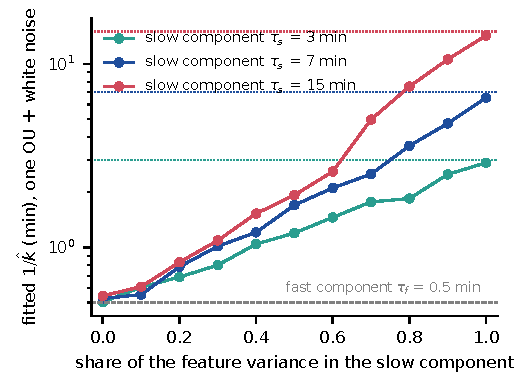
\includegraphics[width=\columnwidth]{fig2_ou_timescale.pdf}
\caption{\textbf{An Ornstein--Uhlenbeck fit returns the dominant time scale of the feature it is given.} A simulated feature is the sum of a fast component ($\tau_f=0.5$~min), a slow component ($\tau_s$ of 3, 7 or 15~min, dotted lines) and white noise, on the OSF 3uszv design (48 sessions of 57~min with probe windows and 10\,\% further epochs missing). It is fitted with one Ornstein--Uhlenbeck process plus white noise, the DMN channel of M1. The fitted time constant moves from $\tau_f$ to $\tau_s$ as the slow component's share of the feature variance grows.}
\label{fig:sim}
\end{figure}
